\chapter{Opis projektnog zadatka}
		
		\textbf{\textit{dio 1. revizije}}\\
		
		\textit{Cilj ovog projekta je razviti programsku podršku za stvaranje web aplikacije „Halo112“. To je aplikacija za olakšavanje koordinacije između rada svih spasilačkih službi. Neregistriranom korisniku se pojavljuje stranica za prijavu. Potrebno je unijeti korisničko ime i lozinku. Ispod polja za unos postoji hiperlink „registriraj se“ – vodi korisnika na stranicu za registraciju.
			Na stranici za registraciju potrebno je unijeti osobne podatke:
		}
		\begin{packed_item}
			\item \textit{korisničko ime}
			\item \textit{lozinka (potrebno je dva puta upisati lozinku na dva različita polja za tekst radi sigurnosti)}
			\item \textit{ime}
			\item \textit{prezime }
			\item \textit{email adresa}
			\item \textit{broj mobitela}
			\item \textit{fotografija(opcionalno)}
		\end{packed_item}
		\textit{Sve osim podataka na kojima piše opcionalno su obavezni za unos, i ne može se nastaviti ako nisu popunjena. Osim osobnih podataka, treba se odabrati i uloga:
		}
		\begin{packed_item}
			\item \textit{dispečer}
			\item \textit{doktor}
			\item \textit{vatrogasac}
			\item \textit{policajac }
		\end{packed_item}
		
		\textbf{\textit{Korisnik}}\\
		\textit{Nakon što je korisnik popunio sva potrebna polja, na dnu stranice postoji gumb „pošalji prijavnicu“. Ako se prelazi mišem preko gumba može se vidjeti: „Administrator mora odobriti vašu prijavu“. Klikom na gumb dešavaju se dvije stvari: administratoru dolazi obavijest o registraciji novog korisnika (on može odobriti ili onemogućiti prijavu i također vidi popis svih ostalih registriranih korisnika), korisnika se šalje na novu stranicu. Na stranici piše: „Obavijestit ćemo vas e-mailom kada administrator odobri vašu prijavnicu.“. Ispod natpisa postoji hiperlink „vrati se na stranicu za prijavu“.}
		
		\textbf{\textit{Administrator}}\\
		\textit{Administratoru se nakon prijave u sustav prikazuje na početnoj stranici prikazuje popis korisnika kojima se čeka potvrda registracije. On može odobriti registraciju ili odbiti, čime će se automatski poslati mail korisniku o odobrenju/otkazanju njegove registracije. Na posebnoj stranici ima popis korisnika u sustavu. Svakom korisniku ima pristup u osobne podatke i podatke o ulozi (dispečer, doktor, vatrogasac ili policajac). Sve od navedenog administrator može promijeniti. Na trećoj stranici postoji popis stanica u gradu koje može dodavati ili brisati.}
		
		\textbf{\textit{Spasioci}}\\
		\textit{Doktori, vatrogasci i policajci su spasioci. Svaki spasilac pripada nekoj stanici (npr. KBC Rebro, PP Trešnjevka, VP Dubrava.) Kojoj stanici pripada bira voditelj te stanice (on je isto spasilac). Spasilac će trebati raditi određene akcije spašavanja, i ponekad neće biti dostupan (izvan radnog vremena, trenutno izvodi drugu akciju). On može ručno namjestit je li spreman ili nije u postavkama profila, a dok izvodi drugu akciju automatski se postavlja da je nespreman za ostale akcije.\\
		Ako spasilac ne izvodi trenutno nikakvu akciju i ako je slobodan prikazuje mu se tablica sa zahtjevima za uključivanje u akcije (Akcije zadaje dispačer u posebnom sučelju). On se može odazvati na jednu od ponuđenih akcija (ako ih uopće ima). Za svaku akciju postoje detalji. Prikazuju se neke opće informacije o opisu problema, kolika je razina hitnosti za obradu akcije i kako bi se spasilac kojemu je zahtjev poslan trebao odazvati (pješke, autom, motorom...). Mogu se prikazati i fotografije. Nakon što se odazvao na neku akciju, ne može odabrati drugu dok ova akcija nije završena ili dok ga dispačer nije uklonio s trenutne akcije.\\
		Spasiteljima koji su aktivni na nekoj akciji na početnoj im se stranici ne prikazuje više tablica ponuđenih akcija, nego mapa grada. Na mapi grada nalazi se sve vezano uz trenutnu akciju, može vidjeti sve ostale spasioce koji trenutno sudjeluju u toj akciji i na karti mu se prikazuju zadaci koje može izvoditi. Svaki zadatak je statičan i prikazuje se na mapi kao točka. Ako se mišem stisne na zadatak mogu se vidjeti detalji zadatka. U detaljima piše kratki komentar što se treba obaviti i kako. Za neke zadatke može se na mapi prikazati ruta, kao put kojim bi spasilac trebao doći do lokacije.
		}
	
		\textbf{\textit{Voditelj Stanice}}\\
		\textit{Voditelj stanice ponaša se isto kao običan spasilac u gotove svemu. Posebno kod njega je što ima posebnu stranicu gdje može odabrati koji spasioci su dio njegove stanice. Također definira na koji su način spasilaci osposobljeni voditi spašavanje. Doktor može biti osposobljen za vožnju motociklom ili kao putnik u kolima hitne pomoći. Vatrogasac može biti osposobljen za vožnju autocisterni, autoljestvi, zapovjednog vozila i šumskog vozila. Policajac se može kretati pješke kao kontaktni policajac, pomoću motocikla, automobila i oklopnog vozila.}
		
		\textbf{\textit{Dispečer}}\\
		\textit{Dispečer na temelju prijave otvara akcije spašavanja s dostupnim informacijama i fotografijama. Dispečer vidi broj dostupnih spasioca po stanicama i može poslati zahtjev za uključivanjem spasilaca u akciju spašavanja. Prilikom slanja zahtjeva dispečer definira na koji način bi spasilac trebao sudjelovati (auto, pješke.. ) i koja je razina hitnosti. Spasioci koji zadovoljavaju kriterije se mogu odazvati na akciju. Dispečer, ako je to potrebno, može spasioca ukloniti s akcije. Ako je akcija spašavanja završila, dispečer je u sustavu može označiti kao gotovom.//
		Dispečer preko karte spasiocima pojedinačno zadaje zadatke. Zadatak može tražiti prolazak određenom rutom i dolazak do određene lokacije. Svaki zadatak može imati i dodatan komentar od dispečera. Za izračun ruta koje prate staze i ceste koristi se vanjski servis OSRM2. //
		Dispečeru se na temelju trenutnih pozicija spasilaca prikazuje Voronojev dijagram. Dispečer može odabrati da se za izradu dijagrama koriste pozicije svih spasioca, ili svih dostupnih neaktivnih spasioca, ili aktivnih spasioca na određenoj akciji. Ovisno o načinu na koji spasilac sudjeluje u akciji, dispečeru se na karti prikazuje drugačija ikona.
		}
	
		\textbf{\textit{Potencijalna korist projekta}}\\
		\textit{Ovaj projekt mogao bi biti od velike koristi bilo kojoj spasilačkoj službi jer jako olakšava komunikaciju između služba. Ako se dogodi nekakva nesreća/problem, puno prije i lakše spasilaci mogu iskomunicirati tko se i gdje treba nalaziti da što prije otklone problem.}
		
		\textbf{\textit{Postojeća slična rješenja}}\\
		\textit{ Slično rješenje u svijetu je belgijska aplikacija "112 BE". "112 BE" je besplatna službena aplikacija belgijskog tima za hitne slučajeve (policija, vatrogasci, hitna pomoć). Nakon registracije u aplikaciju moguće je komentirati službu za korisnike koja uz pomoć vaše lokacije odabire najbliže spasioce koje treba poslati. U ovoj verziji se komunicira preko  interneta no ukoliko nema interneta postoji i mogućnost SMS poruka koja je u ovom slučaju besplatna. Također ukoliko osoba nije u mogućnosti govoriti otvara se chat kako bi se moglo komunicirati  }


		\begin{figure}[H]
			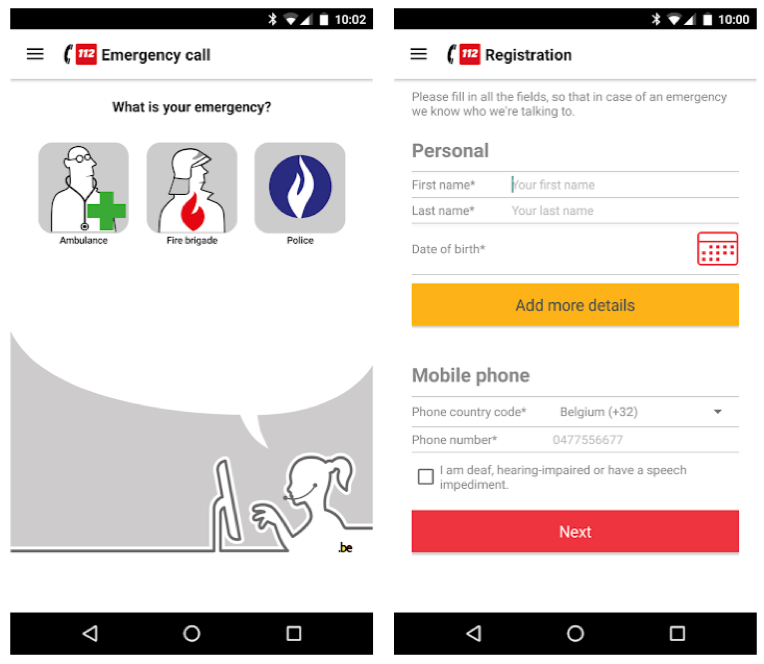
\includegraphics[scale=0.5]{slike/112-app-options.PNG}
			\centering
			\caption{Primjer postojećeg rješenja}
			\label{fig:112_BE}
			\end{figure}
		
		\textbf{\textit{Skup korisnika koji bi mogao biti zainteresiran za ostvareno rješenje}}\\
		\textit{Ovaj projekt može koristiti bilo kakav spasilac. Vrlo vjerojatno bi voditelj stanice određivao bi li se koristila aplikacija ili ne. Ako se odluči da bi aplikacija bila korisna mogao bi ju uvesti kao obavezno sredstvo za komuniciranje između svojih spasilaca. Organizacija bi im se odmah poboljšala.}
		
		\textbf{\textit{Mogućnost prilagodbe rješenja}}\\
		\textit{Ovaj program je jako fleksibilan i može se uvesti jako puno različitih funkcionalnosti. Ako se tijekom izrade programa neka funkcionalnost čini redundantna, može se lako zamjeniti drugom ili ukloniti. Dodatne funkcionalnosti se također vrlo lako mogu dodavati.}
		
		\textbf{\textit{Opseg projektnog zadatka}}\\
		\textit{Ovaj zadatak se može implementirati na bezbroj različitih načina od kojih postoje i teži i lakši načini. Naravno cilj je napraviti ispravan i koristiv program, a ne si olakšavat ili otežavat posao radi posla. Svaku funkcionalnost potrebno je dodati na prvenstveno ispravan način bez nepotrebnog otežavanja zadatka.}
		
		\textbf{\textit{Moguće nadogradnje projektnog zadatka}}\\
		\textit{Ovaj zadatak se može vrlo jednostavno urediti naknadno. Uz ideju nekog voditelja stanice mogle bi se dodati nove funkcionalnosti za tu stanicu ili za sve korisnike.}
		
		
		\eject
		
		
		
		\section{Primjeri u \LaTeX u}
		
		\textit{Ovo potpoglavlje izbrisati.}\\

		U nastavku se nalaze različiti primjeri kako koristiti osnovne funkcionalnosti \LaTeX a koje su potrebne za izradu dokumentacije. Za dodatnu pomoć obratiti se asistentu na projektu ili potražiti upute na sljedećim web sjedištima:
		\begin{itemize}
			\item Upute za izradu diplomskog rada u \LaTeX u - \url{https://www.fer.unizg.hr/_download/repository/LaTeX-upute.pdf}
			\item \LaTeX\ projekt - \url{https://www.latex-project.org/help/}
			\item StackExchange za Tex - \url{https://tex.stackexchange.com/}\\
		
		\end{itemize} 	


		
		\noindent \underbar{podcrtani tekst}, \textbf{podebljani tekst}, 	\textit{nagnuti tekst}\\
		\noindent \normalsize primjer \large primjer \Large primjer \LARGE {primjer} \huge {primjer} \Huge primjer \normalsize
				
		\begin{packed_item}
			
			\item  primjer
			\item  primjer
			\item  primjer
			\item[] \begin{packed_enum}
				\item primjer
				\item[] \begin{packed_enum}
					\item[1.a] primjer
					\item[b] primjer
				\end{packed_enum}
				\item primjer
			\end{packed_enum}
			
		\end{packed_item}
		
		\noindent primjer url-a: \url{https://www.fer.unizg.hr/predmet/proinz/projekt}
		
		\noindent posebni znakovi: \# \$ \% \& \{ \} \_ 
		$|$ $<$ $>$ 
		\^{} 
		\~{} 
		$\backslash$ 
		
		
		\begin{longtblr}[
			label=none,
			entry=none
			]{
				width = \textwidth,
				colspec={|X[8,l]|X[8, l]|X[16, l]|}, 
				rowhead = 1,
			} %definicija širine tablice, širine stupaca, poravnanje i broja redaka naslova tablice
			\hline \multicolumn{3}{|c|}{\textbf{naslov unutar tablice}}	 \\ \hline[3pt]
			\SetCell{LightGreen}IDKorisnik & INT	&  	Lorem ipsum dolor sit amet, consectetur adipiscing elit, sed do eiusmod  	\\ \hline
			korisnickoIme	& VARCHAR &   	\\ \hline 
			email & VARCHAR &   \\ \hline 
			ime & VARCHAR	&  		\\ \hline 
			\SetCell{LightBlue} primjer	& VARCHAR &   	\\ \hline 
		\end{longtblr}
		

		\begin{longtblr}[
				caption = {Naslov s referencom izvan tablice},
				entry = {Short Caption},
			]{
				width = \textwidth, 
				colspec = {|X[8,l]|X[8,l]|X[16,l]|}, 
				rowhead = 1,
			}
			\hline
			\SetCell{LightGreen}IDKorisnik & INT	&  	Lorem ipsum dolor sit amet, consectetur adipiscing elit, sed do eiusmod  	\\ \hline
			korisnickoIme	& VARCHAR &   	\\ \hline 
			email & VARCHAR &   \\ \hline 
			ime & VARCHAR	&  		\\ \hline 
			\SetCell{LightBlue} primjer	& VARCHAR &   	\\ \hline 
		\end{longtblr}
	


		
		
		%unos slike
		\begin{figure}[H]
			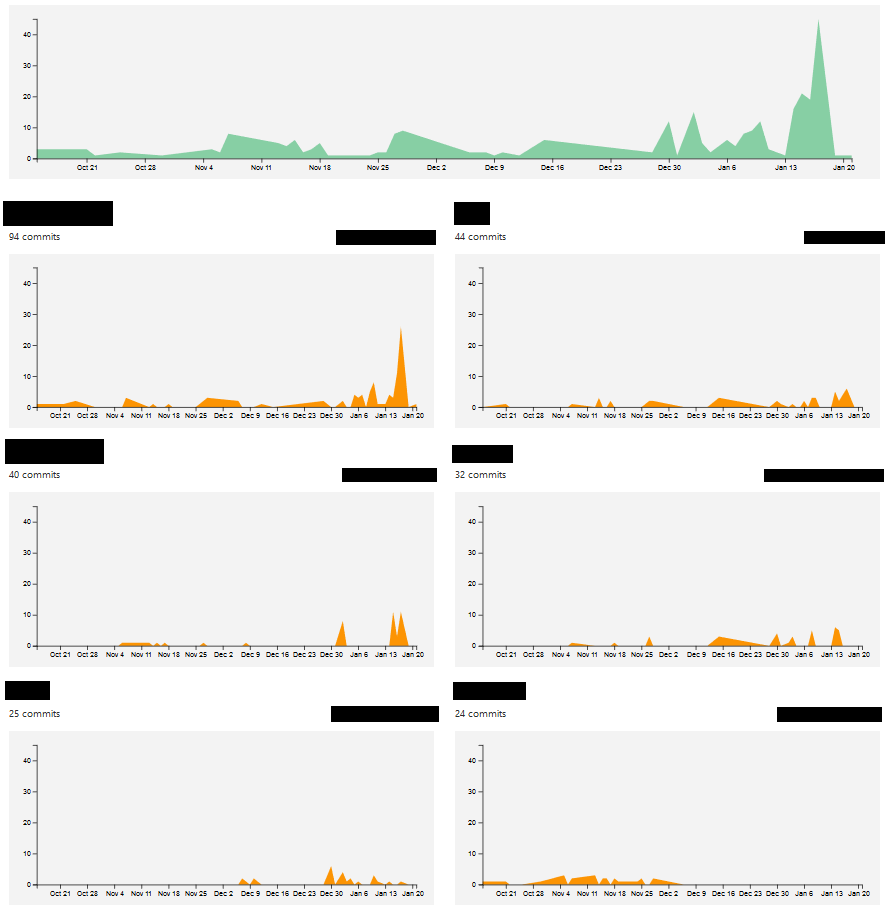
\includegraphics[scale=0.4]{slike/aktivnost.PNG} %veličina slike u odnosu na originalnu datoteku i pozicija slike
			\centering
			\caption{Primjer slike s potpisom}
			\label{fig:promjene}
		\end{figure}
		
		\begin{figure}[H]
			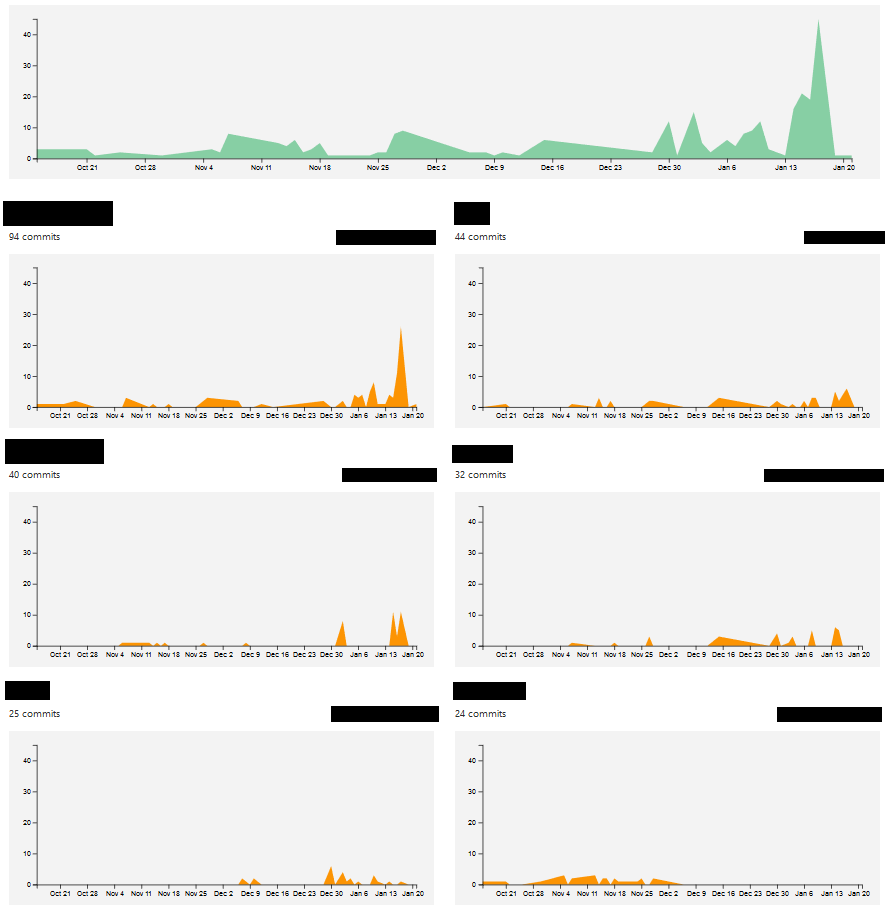
\includegraphics[width=\textwidth]{slike/aktivnost.PNG} %veličina u odnosu na širinu linije
			\caption{Primjer slike s potpisom 2}
			\label{fig:promjene2} %label mora biti drugaciji za svaku sliku
		\end{figure}
		
		Referenciranje slike \ref{fig:promjene2} u tekstu.
		
		\eject
		
	